\section{Interaktive Karte}
 [TODO] intro
- talk about google map

\subsection{Leistung bei der Datenerfassung}

Die interaktive Karte verdankt ihre Langsamkeit vor allem dem Abruf der Sensordaten, der über mehrere Aufrufe an eine sehr langsame API erfolgt.
Tatsächlich dauert es mehr als 2000 Millisekunden, um einfach nur den Standort von 10 Sensoren an einem Standort abzurufen.
Der Grund dafür ist, dass der Backend Service viele Informationen über die Sensoren zurückgibt, was wiederum umfangreiche JOINs in der Datenbank erforderlich macht.

\begin{figure}[H]
  \centering
  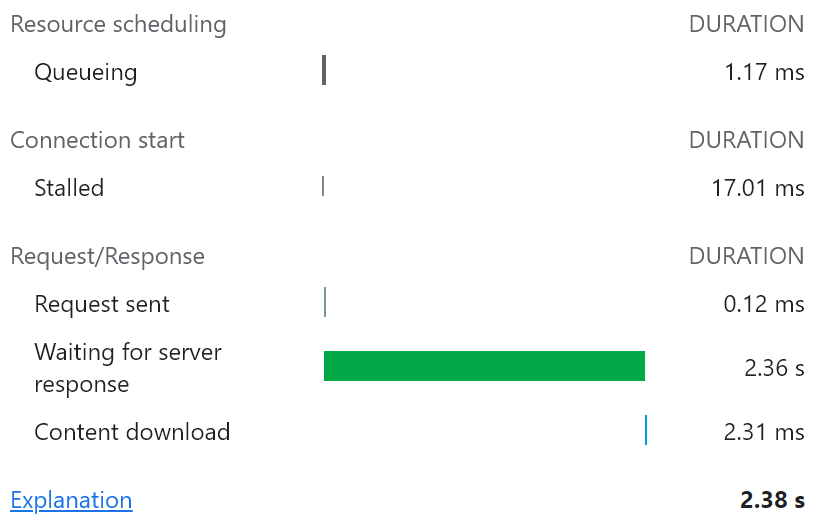
\includegraphics[width=8cm]{api_sensors_global_duration}
  \caption{Durchschnittliche Antwortzeit bei 10 Aufrufen an die Sensor-API}
  \label{fig:api_sensors_global_duration}
\end{figure}

Die Anwendung muss dann für jeden Sensor einen weiteren API-Aufruf tätigen, um dessen Status abzurufen.
Diese Strategie ist für eine interaktive Karte nicht geeignet, da das Hinzufügen von Sensoren die API noch weiter verlangsamen würde.
Es ist eine neue Strategie erforderlich, die es ermöglicht, den Standort und den Status von Tausenden von Sensoren innerhalb einer angemessenen Zeit abzurufen.

Drei Hauptideen wurden ausgewählt.
Da diese Techniken nicht zum direkten Thema der Thesis gehören, werden sie nur kurz beschrieben.

\subsubsection{API-Antwort-Cache}

Der Großteil der derzeit verfügbaren APIs implementiert ein Caching-System für Antworten\cite{redis}.
Wenn ein Benutzer eine Liste aller Sensoren an einem bestimmten \textit{Site} anfordert, wird die Antwort mit einem \ac{TTL} gespeichert und der nächste Benutzer, der die gleiche Liste anfordert, erhält die Antwort aus dem Backup, wenn der \ac{TTL} nicht abgelaufen ist.

\paragraph{Vorteile}
\begin{itemize}
  \item Verringerung der Serverbelastung
  \item Einfache Einrichtung mit ID-basierten Speichersystemen wie z.B. Redis
  \item Kann auf Browserseite im Header der \ac{HTTP}-Antwort einer Anfrage verwaltet werden
\end{itemize}

\paragraph{Nachteile}
\begin{itemize}
  \item Die Antworten sind schneller, aber sie lösen nicht die Tatsache, dass der Benutzer dann für jeden Sensor eine neue Anfrage aufrufen muss
  \item Kann nicht auf der Clientseite implementiert werden, da es zu Inkonsistenzen bei den kritischen Client-Server-Daten kommen kann (Feuer entdeckt)
\end{itemize}

\subsubsection{API mit serverseitiger Statusberechnung} \label{sec:API_serverseitiger_Statusberechnung}

Dieser Ansatz zielt darauf ab, zwei neue API-Endpunkte speziell für die Karte zu erstellen, die den Standort und den Status der \textit{Sites} und die Sensoren eines \textit{Site} abrufen können.

\paragraph{Vorteile}
\begin{itemize}
  \item Relativ einfach einzurichten, ohne Breaking Changes zu verursachen
  \item Der Kunde muss nicht mehr die API aufrufen, um den Status jedes einzelnen Sensors abzufragen, sondern es genügen zwei Anfragen.
\end{itemize}

\paragraph{Nachteile}
\begin{itemize}
  \item fügt hyperspezifische Endpunkte hinzu, wodurch die API komplizierter zu verstehen ist
  \item Die Berechnung des Status eines Sensors ist auf der Serverseite schneller, aber je mehr Sensoren vorhanden sind, desto langsamer ist die Antwort
\end{itemize}

\subsubsection{Kontinuierliche Berechnung mit Big-Data-Ansatz} \label{sec:API_bigdata}

Diese Technik implementiert die vorherige Technik (siehe \ref{sec:API_serverseitiger_Statusberechnung}), außer dass die Berechnung des Status eines bestimmten Sensors in einer temporären Datenbanktabelle gespeichert wird.
Sobald ein Sensor eine Information sendet, wird sein Status parallel zum Hauptprozess neu berechnet und der Eintrag in der Datenbank geändert.
So wird die Abfrage des Status der Sensoren einer \textit{Site} einfach zum Lesen einer Datenbanktabelle.

\paragraph{Vorteile}
\begin{itemize}
  \item Extrem schnelle Antwortzeit, da keine Datenverarbeitung erforderlich ist
  \item Ressourceneffizienz, da die Berechnungen nur für ein bestimmtes Element bei einem bestimmten Ereignis durchgeführt werden
  \item Kann in einer Micro-Service-Architektur isoliert werden
\end{itemize}

\paragraph{Nachteile}
\begin{itemize}
  \item Erfordert einen Fallback, um sicherzustellen, dass die Daten mit der Datenbank konsistent sind
  \item Höhere Entwicklungskosten
\end{itemize}

\subsubsection{Entscheidung}

Zusammen mit dem Backend-Team wurde beschlossen, die letzte Option (siehe \ref{sec:API_bigdata}) in der nächsten Version der Anwendung zu implementieren.
Aus Zeit- und Prioritätsgründen wird jedoch die zweite Option (siehe \ref{sec:API_serverseitiger_Statusberechnung}) implementiert.
Die Nutzung der API ist die gleiche, aber die Leistung ist nicht optimal.

Dadurch konnte die Anzahl der API-Aufrufe, die zuvor linear zur Anzahl der Sensoren an einem Standort war, auf eins reduziert werden.
Die Reaktionszeit ist mit über 1100 Millisekunden für 10 Sensoren immer noch übermäßig hoch, aber diese Lösung ist nur eine Übergangslösung und für die Größe der derzeit in Produktion befindlichen Sites immer noch verwendbar.

\begin{figure}[H]
  \centering
  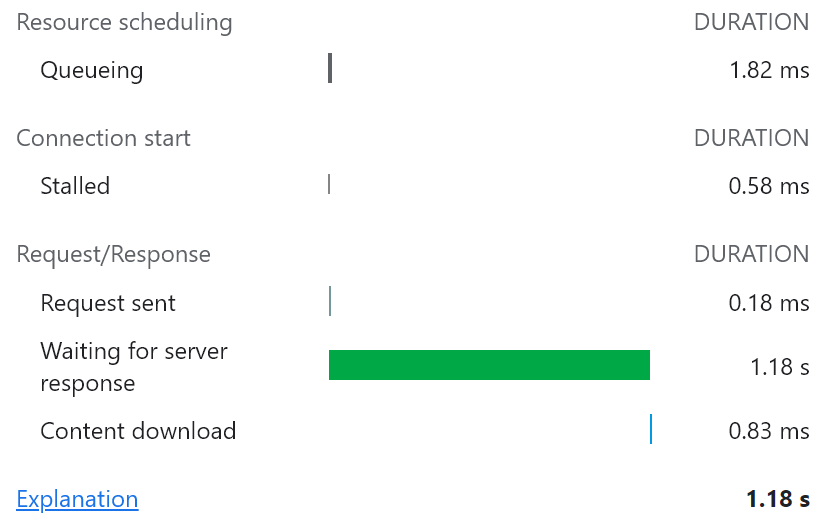
\includegraphics[width=8cm]{api_sensors_map_duration}
  \caption{Durchschnittliche Reaktionszeit für 10 API-Aufrufe, die der Anzeige von Sensoren auf der Karte zugedacht sind}
  \label{fig:api_sensors_map_duration}
\end{figure}

Das Detail der neuen API, das für die Karte gewidmet ist, finden Sie im Anhang \ref{appendix:map-api}.

\subsection{Clustering von \textit{Sites} und Sensoren}

Die Tatsache, dass es zwei mögliche Ebenen von Clustern zwischen \textit{Sites} und Sensoren gibt, erlaubt es nicht, das native Clustering-API von Google Maps zu verwenden, das nur für Punkte mit der gleichen Hierarchie funktioniert.
Wir müssen also die Clustering-Logik selbst entwickeln, indem wir den \ref{fig:map_clustering_flow} flow implementieren.
